\documentclass[svgnames,tikz]{standalone}
\usepackage{pgfmath}
\usetikzlibrary{positioning,arrows,calc,3d}

\tikzset{
  focus/.style args={#1 at #2}{
    insert path={
      %{ [white] (#2.north east) rectangle (#2.south west)}
      ($(#2.center)!#1!(#2.north east) $) rectangle ($(#2.center)!#1!(#2.south west) $)
    }
  },
  focusout/.style args={#1 at #2}{
    even odd rule,
    insert path={
      (#2.north east) rectangle (#2.south west)
      ($(#2.center)!#1!(#2.north east) $) rectangle ($(#2.center)!#1!(#2.south west) $)
    }
  },
  txt/.style={font=\Large\tt},
  img/.style={
     inner sep=2pt,
     draw,
     label/.append style={font=\small\tt},
  },
}


\begin{document}
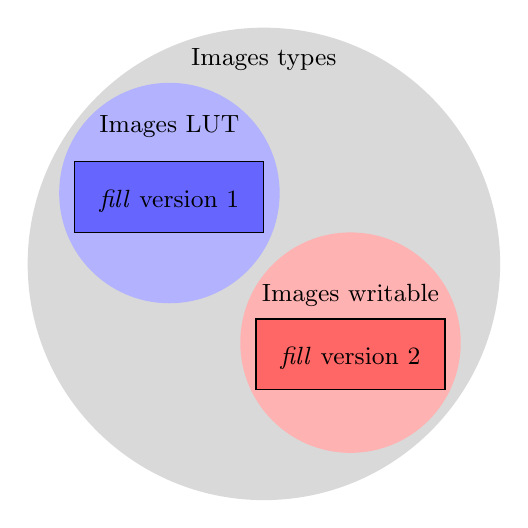
\begin{tikzpicture}
  \tikzset{every node/.style={node distance=5pt, font=\small}}

  \begin{scope}
    \fill[gray!30!white]  (0, 0)      circle  (3);
    \fill[blue!30!white]  (-1.2, 0.9) circle  (1.4);
    \fill[red!30!white]   (1.1, -1)   circle  (1.4);

    \draw[black, fill=blue!60!white]  (-2.4, 1.3)   rectangle (0, 0.4);
    \draw[black, fill=red!60!white]   (-0.1, -0.7)  rectangle (2.3,-1.6);
  \end{scope}

  \node at (0, 2.6)       {Images types};

  \node at (-1.2, 1.75)   {Images LUT};
  \node at (-1.2, 0.8)    {\emph{fill} version 1};

  \node at (1.1, -0.4)    {Images writable};
  \node at (1.1, -1.2)    {\emph{fill} version 2};

\end{tikzpicture}
\end{document}